\documentclass[]{article}
\usepackage{styl-notatek}
\begin{document}
\onehalfspacing
\begin{titlepage} 
    \begin{center}
         \begin{figure}[h]
            \centering
            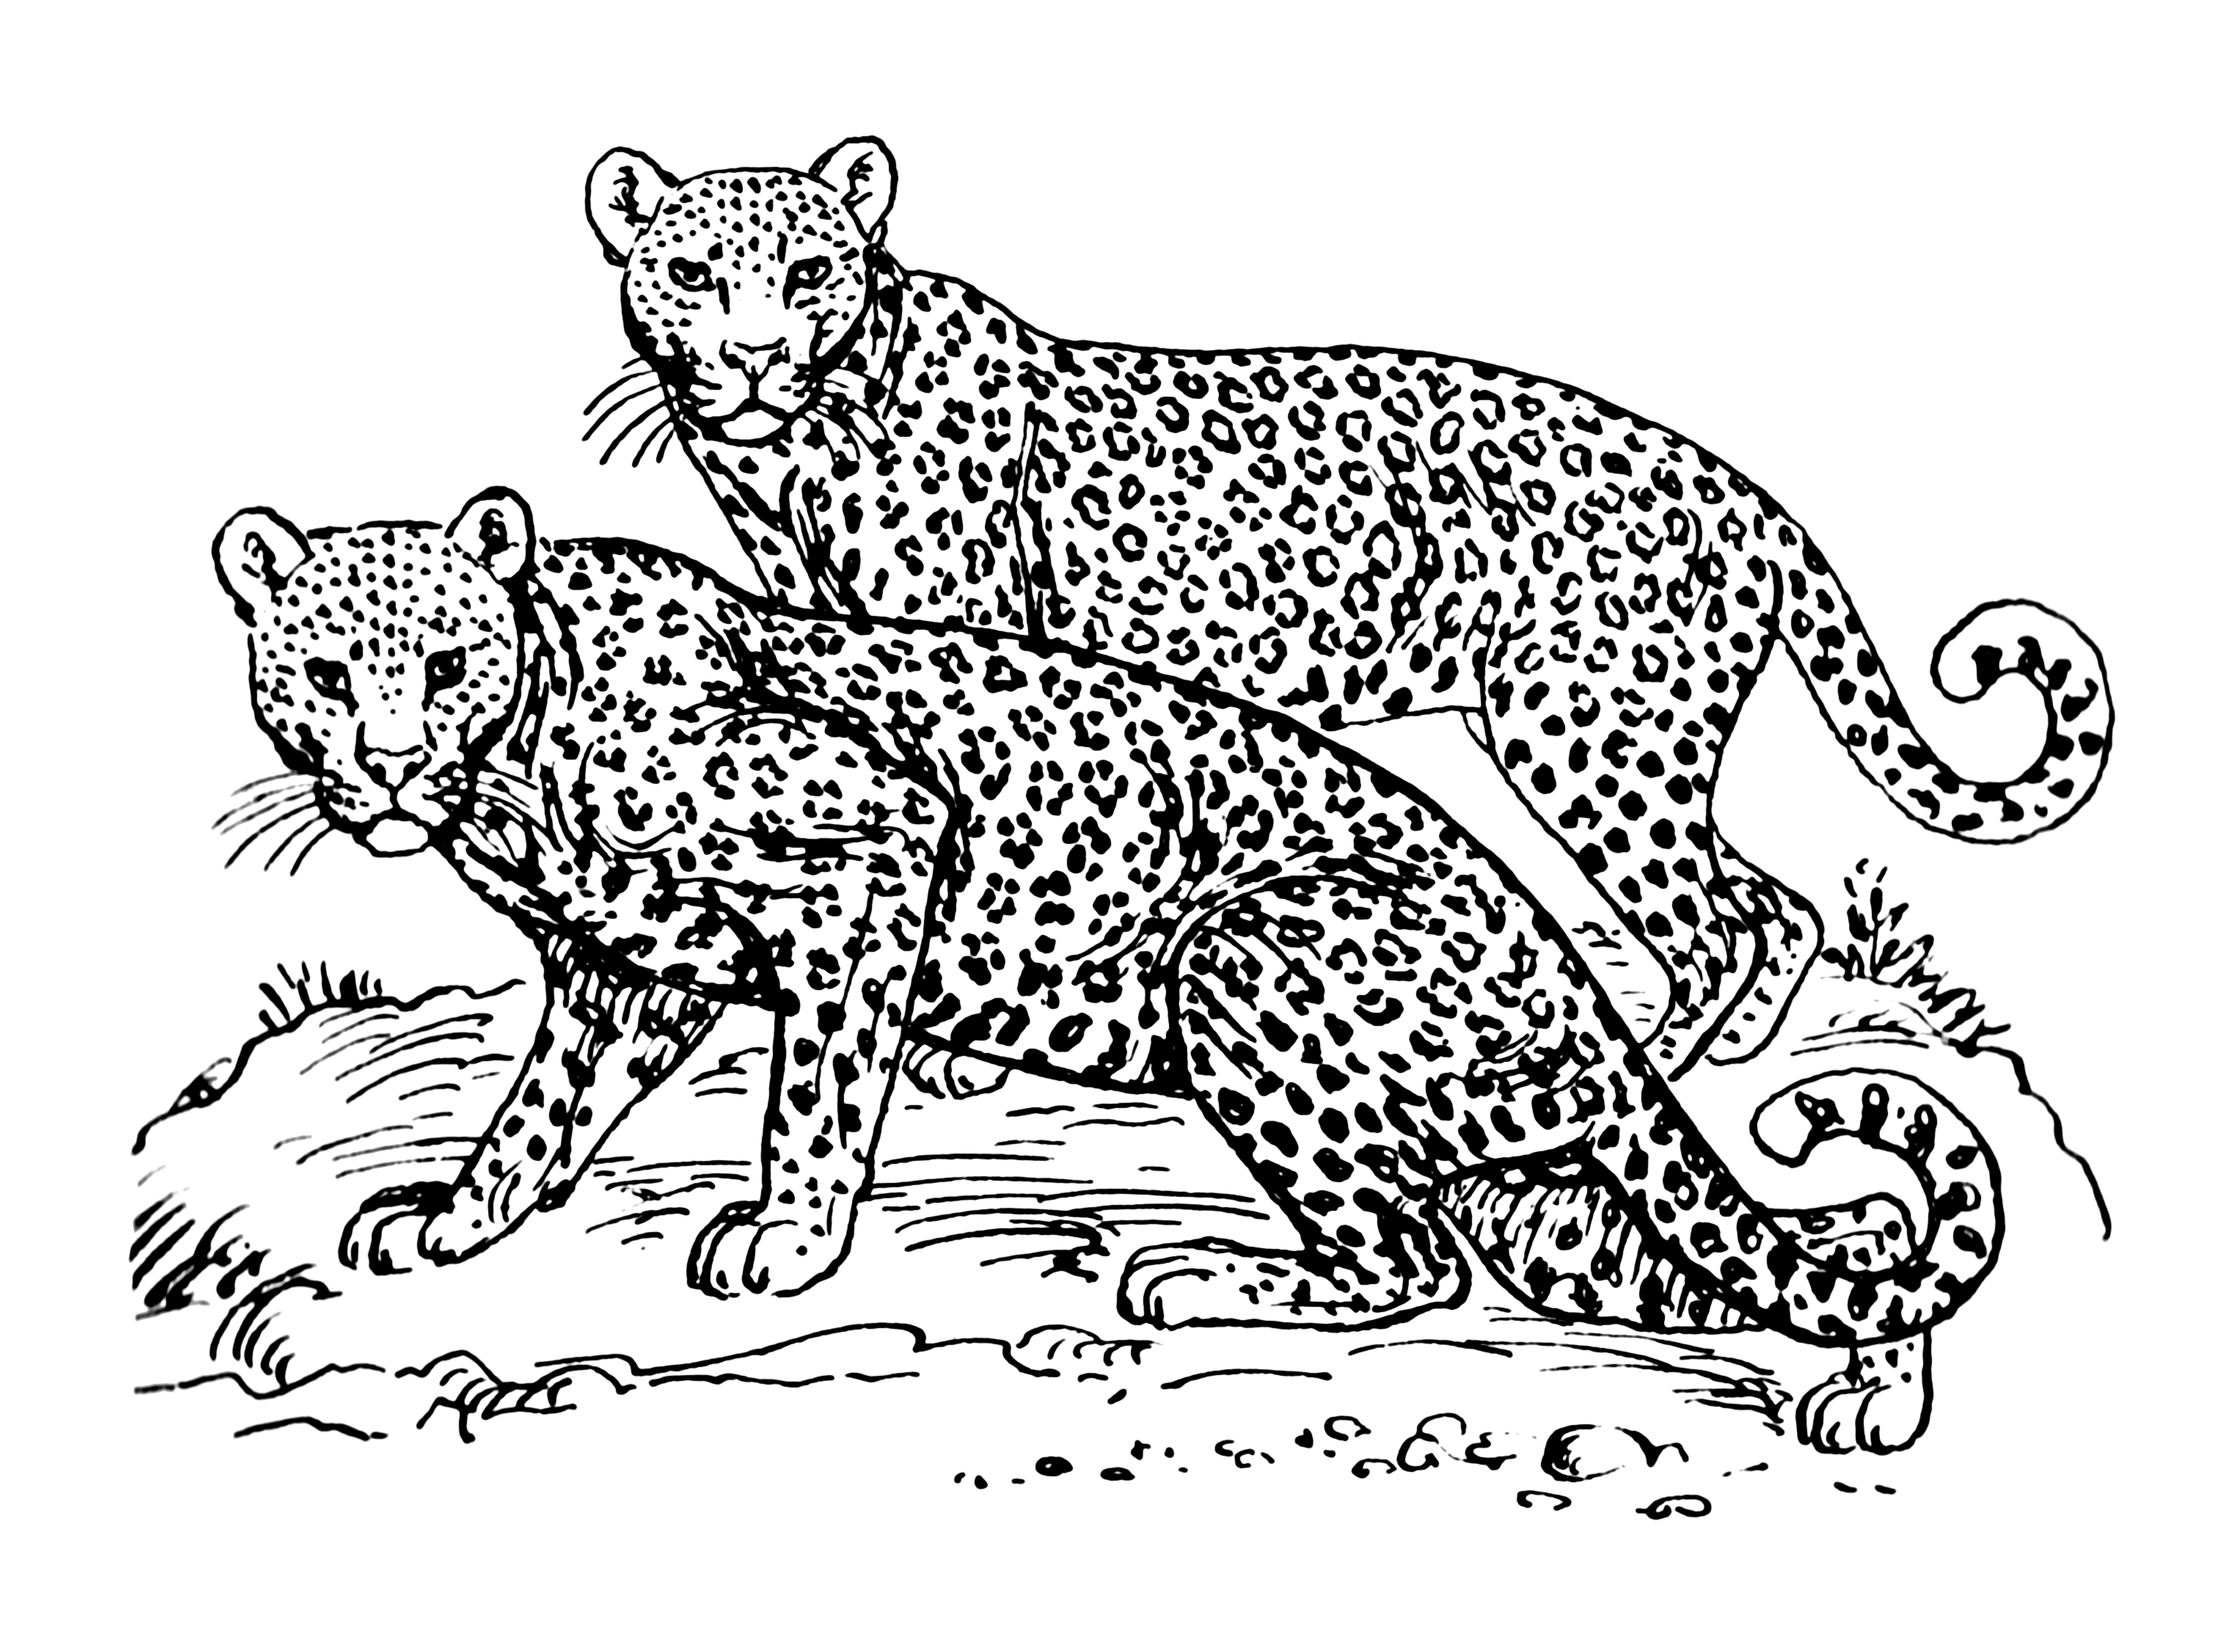
\includegraphics[]{img/pumy.png}
           
        \end{figure}
        
        \Huge
        \textbf{\textsc{Metody Probabilistyczne \\ w Uczeniu Maszynowym}}
        
        \vspace{0.5cm}
        \Large
        \textsc{Zagadnienia Egzaminacyjne}
        \line(1,0){330}
        
        \normalsize
        
        \vspace{1cm}
        \textit{,,Gdzie błąd?''}
        \vspace{1cm}

        \textit{\textsc{Popełnione przez}}\\
        \vspace{5mm}
  
        \textbf{\textsc{Załatany Ponton}}
 
        \vfill

        Kraków \\
        Anno Domini 2023
    \end{center}
\end{titlepage}
\fancyhead[L]{\textbf{\textit{SK}}}
\fancyhead[C]{\thepage}
\fancyhead[R]{
\includegraphics[width=1cm]{tcs.png}}
\tableofcontents
\section{Teoria sygnałów}
\subsection{Twierdzenie Fouriera}
    Rozsądne funkcje okresowe wyrażają się szeregiem funkcji trygonometrycznych.
   \[ f(x) = c_0 + \sum_{i=1}^{\infty} a_i \sin(i \cdot x) + \sum_{i=1}^{\infty} b_i \cos(i \cdot x) \]
gdzie
\[ c_0 = \frac{1}{2\pi} \int_{-\pi}^{\pi} f(x) \, dx \]
\[ a_i = \frac{1}{\pi} \int_{-\pi}^{\pi} f(x) \sin(i \cdot x) \, dx \]
\[ b_i = \frac{1}{\pi} \int_{-\pi}^{\pi} f(x) \cos(i \cdot x) \, dx \]

\subsection{Twierdzenie Nyquista}
Jeżeli funkcja f nie ma składowych o częstotliwościach większych niż $B$  Hz i próbkujemy ją z częstotliwością $2B$ Hz, to możemy jednoznacznie odtworzyć f.
    
\noindent
Maksymalna przepustowość, to $2B\log\sum$, gdzie $\sum$ to liczba bitów w każdej próbce.
\subsection{Twierdzenie Shannona}
Jeżeli S/N to stosunek mocy sygnału do mocy szumu, to maksymalna przepustowość, to \linebreak $B\log(1+S/N)$.
\newpage
\section{Model ISO-OSI i TCP/IP}
\subsection{Model ISO-OSI?}
Open System Interconnection Reference Model - jest traktowany jako wzorzec dla większości rodzin protokołów komunikacyjnych, jego podstawowym założeniem jest podział systemów sieciowych na 7 warstw:
\begin{itemize}
    \item Warstwa fizyczna \\
    transmisja danych pomiędzy węzłami sieci, połączenia mechaniczne, przewody elektryczne, karty sieciowe, koncentratory
    \item Warstwa łącza danych \\
    kontrola błędów podczas przesyłania, kompresja danych, mosty, przełączniki, sterowniki kart sieciowych
    \item \hyperref[sec:warstwa-sieci]{Warstwa sieci} \\
    ustanawianie, utrzymywanie i rozłączanie połączenia, wyznaczanie optymalnej trasy dla połączenia (trasowanie), rutery
    \item Warstwa transportowa \\
    dbanie o kolejność pakietów otrzymywanych przez odbiorcę, zapewnianie retransmisji w przypadku problemów
    \item Warstwa sesji \\
    nawiązywanie i zrywanie połączenia przez aplikację, realizacja zapytania o usługę (coś jak obsługa API)
    \item Warstwa prezentacji \\
    tłumaczenie danych, definiowanie formatu i odpowiedniej składni, przekształcanie danych na postać standardową, rozwiązywanie problemów z niezgodnymi reprezentacjami
    \item Warstwa aplikacji \\
    zapewnianie aplikacjom metod dostępu do środowiska OSI
\end{itemize}

\subsection{Czym jest TCP/IP?}
Uproszczony, 4 warstwowy model ISO-OPI
\begin{itemize}
    \item Warstwa dostępu do sieci \\
    umieszczanie pakietów TCP/IP w nośniku sieciowym i ich odbiór z nośnika
    \item Warstwa internetu \\
    adresowanie, pakowanie i funkcje routowania
    \item Warstwa transportowa \\
    dostarczanie warstwie aplikacji usług sesji i data-gramowych (TCP i UDP)
    \item Warstwa aplikacji \\
    umożliwienie aplikacjom korzystania z usług innych warstw
\end{itemize}

\begin{figure}[H]
    \centering
    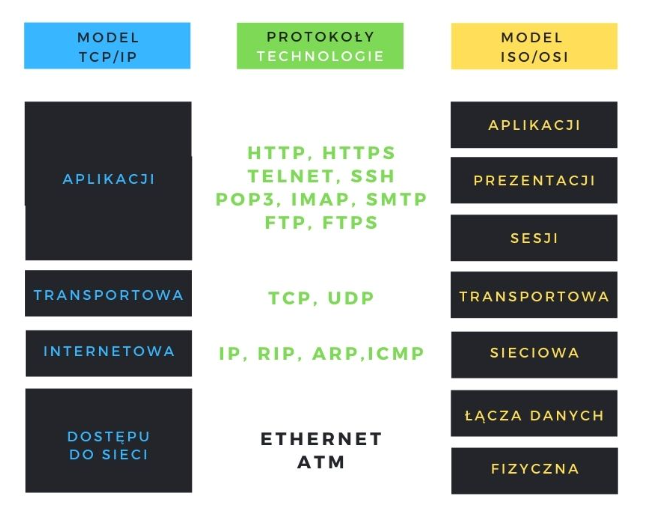
\includegraphics[width=0.7\textwidth]{model.png}
    {\tiny https://ti.nstrefa.pl/wp-content/uploads/2020/11/protokoly-modelu-sieci.jpg}
\end{figure}

\subsection{Nadawanie większych komunikatów}
\subsubsection{Sposoby synchronizacji zegara}
\textbf{Manchester} \\
Zmiana sygnału w połowie każdego bitu \\
1 $\rightarrow$ 10 \\
0 $\rightarrow$ 01 \\
Jest odporny na zmiany szybkości transmisji i dobrze radzi sobie z długimi ciągami jednakowych bitów, wadą jest, to że trzeba używać dwukrotnie szerszego pasma przez to, że jest zmiana sygnału na początku bitu, gdy poprzedni był taki sam.\\\\
\textbf{NRZI (Non-Return to Zero Invert)} \\
Zmiana sygnału koduje 0, brak zmiany koduje 1. Nie daje sobie rady dla długich ciągów 0, bo może wtedy wystąpić desynchronizacja, dlatego zwykle używa się go łącznie z inną metodą synchronizacji, która zapewnia, że takie ciągi nie wystąpią takie jak:
\begin{itemize}
    \item \textbf{4B/5B}
    Zamienia każdy 4 bitowy segment informacji w 5 bitowy segment według odpowiedniego klucza, zapewniając, że w każdym 5 bitowym segmencie znajdą się przynajmniej 2 jedynki.
    \item \textbf{8B/10B}
    Analogiczne do 4B/5B, ale dodatkowo ilość 1 i 0 jest bardziej równomierna, różnica max 1 na segment, gdzie dla 4B/5B jest to 3 na segment
    \item \textbf{64B/66B}
    Analogicznie do poprzednich, ale rośnie pokrycie łącza, używamy 97\% łącza do komunikacji, zamiast 80\%
    \item \textbf{Random Scrambling}
    Równoważy liczbę 0 i 1
\end{itemize}

\subsection{Niwelowanie błędów komunikacji}
\textbf{Parity bit} \\
Sprawdzenie parzystości, ostatni bit notuje, czy ilość jedynek w poprzednich jest parzysta \\ \\
\textbf{CRC (Cyclic Redundancy Check)} \\
Obliczany poprzez dzielenie ciągu po dopisaniu do niego tylu zer, ile jest bitów w wielomianie. \\
$11010 \rightarrow x^4 + x^3 + x$ wielomian stopnia 4 \\
Ponieważ pomijamy początkowe zera, to taki sam kod zostanie wygenerowany dla danych mających inną liczbę zer na początku. W Ethernecie używany był CRC32, który używa 33 bitowego dzielnika \\ \\
\textbf{Kody korygujące} \\
Kody Hamminga pozwalają nie tylko sprawdzić, czy wiadomość jest poprawna, ale także ją skorygować, potrzebujemy dużo nadmiarowości, ale czasem warto.\\
\\
\textbf{Haszowanie}
\subsection{Potwierdzanie komunikacji}
\subsection{Strategie współdzielenia kanału komunikacji}
\begin{itemize}
    \item ALOHA \\
    wyślij $\rightarrow$ poczekaj $\rightarrow$ jeśli nie ma potwierdzenia, wyślij jeszcze raz
    \item slotted ALOHA \\
    Kanał jest podzielony na krótkie odcinki czasu i można zacząć nadawanie tylko na początku odcinka.
    \item CSMA/CD (Carrier Sense Multiple Access with Collision Detection) \\
    nasłuchuj $\rightarrow$ jeśli nikt nie nadaje, to wyślij dane $\rightarrow$ jeśli była kolizja, wyślij sygnał o kolizji.
    \item Exponential Backoff \\
    * kolizja * $\rightarrow$ wylosuj liczbę odcinków czasu $\rightarrow$ poczekaj $\rightarrow$ wyślij ponownie, po $i$ kolizjach losujemy liczbę z przedziału $[0, 2^i]$
    \item Tokeny \\
    otrzymaj token $\rightarrow$ wyślij wiadomość
\end{itemize}

\section {Ethernet}
\subsection{Historia rozwoju}
Ethernet został stworzony przez Boba Metcalfe kiedy to pracował on nad rozwojem systemu ALOHA, stworzono wtedy metodę wykrywania kolizji poprzez CSMA/CD. Pierwsza wersja powstała na bazie ALOHA w 1973 roku, ale oficjalnie opublikowana została dopiero w 1980, osiągał wtedy maksymalną przepustowość 2,94Mb/s. Później przez wiele lat udoskonalany, w 2022 roku Metcalfe dostał za ten wynalazek Nagrodę Turinga.
\subsection{Ramka}
Nagłówek (7 x 10101010 + 10101011) \\
Adres odbiorcy (6) \\
Adres nadawcy (6) \\
Typ protokołu / długość komunikatu (2) \\
Dane (46-1500) \ 
Suma kontrolna (4) \\
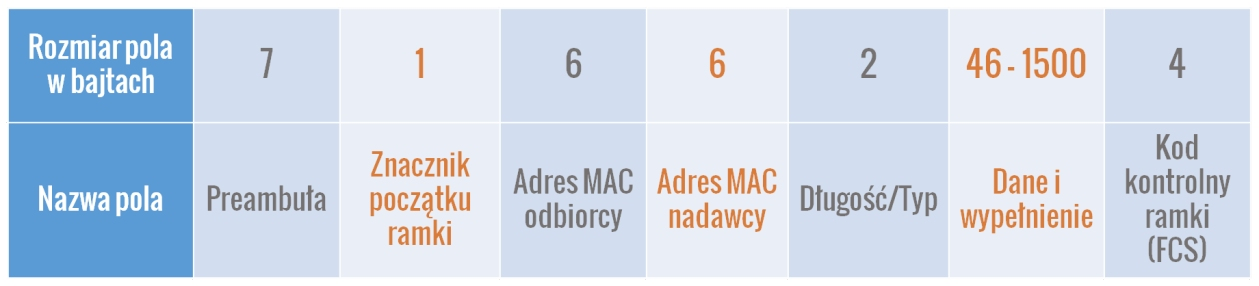
\includegraphics[width=0.7\textwidth]{ramka-ethernetowa.jpg}
\subsection{Szczegóły Ethernetu}
\begin{itemize}
    \item Adres MAC \\
    Unikalny adres urządzenia fizycznego zapisywany w postaci XX:XX:XX:XX:XX:XX
    \item Broadcast \\
    FF:FF:FF:FF:FF:FF szesnastkowo transmituje wiadomość do wszystkich
    \item Protokół ARP (Address Resolution Protocol) \\
    Wysyłane jest zapytanie z adresem docelowym i adresem pytającego. Odpowiada na nie tylko host o adresie podanym w zapytaniu.
    \item Switche
    Pośredniczy w komunikacji pomiędzy urządzeniami.
    \item Cykle
    \item VLAN (wirtualna sieć lokalna) \\
    Fizyczna sieć podzielona na logiczne segmenty na poziomie drugiej warstwy.
\end{itemize}
\subsection{Switched Ethernet}
Z czasem wymyślono przełączniki (switchę), które pozwalają na segmentację sieci co znacznie usprawniło działanie Ethernetu. Przełączniki mają przekazywać ramki między urządzaniami sieciowymi, analizują otrzymaną ramkę i przesyłają ją tylko do portu docelowego. Mechanizm ten pozwala na minimalizowanie liczby kolizji przy zachowaniu przy zachowaniu wszechstronnego połączenia.
\subsection{Cykle}
Cykle w sieci mogą powodować zatory, komunikacja może podróżować w kółko co bez odpowiednich środków zaradczych spowoduje przeciążenie, w dodatku podczas cyklenia się adresy mac mogą być nieprawidłowo aktualizowane. Lepiej unikać.
\subsection{VLAN}
VLAN - (z ang. Virtual Local Area Network) pozwala na segmentację sieci LAN na mniejsze, urządzenia wewnątrz danego vlanu mogą się ze sobą bezpośrednio komunikować, natomiast żeby się skomunikować z urządzeniem z poza swojego vlanu trzeba przejść przez router.
\section{Sieci mobilne}
\subsection{Wi-Fi}
Wi-FI to standard bezprzewodowej radiowej komunikacji. Buduje się w niej wirtualne sieci lokalne oparte na routerach, przez które urządzenia się komunikują. Maksymalna przepustowość to około 1000Mbit/s.
\subsubsection{wykrywanie kolizji}
w technologiach radiowych niemożliwe jest wykrywanie kolizji podczas przesyłu, więc WI-FI nasłuchuje tylko na początku czy coś jest wysyłane i zaczyna wysyłać dopiero jak jest wolne, nie może przerwać w trakcie, później używa
potwierdzeń, aby ustalić czy transmisja się udała.
\subsubsection{Podłączanie się}
Chcąc podłączyć się do sieci Wi-FI urządzenie nasłuchuje wysyłanych periodycznie przez punkty dostępowe Beacon Frame'ów, które zawierają informacje o sieci. Klient informuje punkt dostępu o chęci komunikacji i następuję negocjacja zabezpieczeń (jeśli sieć jest zabezpieczona). Większość sieci jest zabezpieczona protokołami WPA lub WPA2. Wymieniają one wtedy klucze uwierzytelniające i jeśli są one poprawne ustalane są klucze, które będą używane do komunikacji między urządzeniami. W WPA używa się do tego 4 way handshake'ów. Ustalany jest adres IP podłączonego urządzenia i można zacząć komunikacje.
\subsubsection{Point to Point Wi-FI}
Point to Point Wi-Fi to bezprzewodowa metoda rozprzestrzeniania łączności internetowej na dużych obszarach bez konieczności stosowania rozbudowanego okablowania. Osiąga się to poprzez utworzenie pojedynczego szybkiego łącza w optymalnej lokalizacji oraz wykorzystanie anten i sprzętu radiowego PtP do skonfigurowania dodatkowych punktów połączeń.
\susubsection{WiFi + Ethernet}
Połączenie Wi-Fi i internetu polega odbywa się przez punkt dostępowy. Punkt dostępowy jest podłączony kablem do sieci Ethernet i umożliwia on komunikację urządzenia do niego podłączonym.
\subsection{Sieci komórkowe}
\subsection{Problemy z komunikacją}
\begin{itemize}
    \item Słabnący sygnał
    \item Zakłócenia
    \item Auto-zakłócenia
    \item Problemy z obserwacją innych użytkowników
    \item Problem ukrytej stacji \\
    Do stacji nie docierają sygnały, które powstrzymałyby ją od wysłania wiadomości, a które docierają do odbiorcy i zakłócają przesył.
    \item Problem eksponowanej stacji \\
    Sygnały z innej stacji dosięgają tej, przez co powstrzymuje się ona od wysłania wiadomości, choć niesłusznie, bo nie docierają one do adresata.
    \item Kształtowanie wiązki \\
    Kierowanie sygnału Wi-Fi w określonym kierunku (nie we wszystkich kierunkach jak router).
    \item QAM w WiFi (Quadrature Amplitude Modulation) \\
    Tłumaczy cyfrowe paczki danych na sygnał analogowy.
\end{itemize}

\subsection{Role punktów dostępu}
\begin{itemize}
    \item AP (Access Point) w WiFi \\
    Wzmacnia sygnał z rutera
    \item BTS w GSM (Base Transceiver Station) \\
    Stacja bazowa w systemie radiotelefonii Global System for Mobile Telecommunication (standard telefonii komórkowej)
    \item Nawiązywanie połączenia
    \item Sterowanie komunikacją
    \item Przekazywanie połączenia
    \item Bezpieczeństwo
\end{itemize}

\subsection{Kontrola przepływu}
W zależności od protokołu podczas transmisji często konieczne jest wysłanie specjalnej wiadomości informującej drugą stronę o stanie transmisji np.:
\begin{itemize}
\item \textbf{ACK (Acknowledgement)} - wiadomość z potwierdzeniem dostarczenia poprawnej wiadomości wysyłana przez odbiorcę.
\item \textbf{ARQ (Automatic Repeat Request / Query)} - retransmituje wiadomość, jeśli ACK nie przyszło przed upływem określonego czasu. Używane w przypadku zmiennej lub nieznanej przepustowości.
\item\textbf{LDCP (Low-Density Parity Check)} - kody wyznaczane liniowo, które pozwalają na wykrywanie błędów w wiadomościach rzadkich
\item \textbf{RTS i CTS (request to send / clear to send)} - opcjonalny mechanizm rozwiązujący problem ukrytej stacji. Działa, jeśli urządzenia z niego korzystają. Jest wykorzystywany przy przesyłaniu dużych paczek danych.
\end{itemize}
\subsection{Bezpieczeństwo WiFi}
\begin{itemize}
    \item Szyfrowanie kluczem symetrycznym AES (Advanced Encryption Standard) \\
    to algorytm symetrycznego szyfru blokowego o rozmiarze porcji wynoszącym 128 bitów. Konwertuje pojedyncze bloki przy użyciu kluczy o długości 128, 192 i 256 bitów. Po zaszyfrowaniu tych bloków łączy je ze sobą, tworząc zaszyfrowany tekst. \\
    tekst + tajny klucz $\rightarrow$ szyfr $\rightarrow$ zaszyfrowany tekst
    \item CCMP (Counter Mode with Cipher Block Chaining Message Authentication Code Protocol) \\
    to protokół szyfrowania stanowiący część standardu dla bezprzewodowych sieci lokalnych (WLAN). CCMP używa szyfru AES do szyfrowania wrażliwych danych. Wykorzystuje 128-bitowe klucze i 48-bitowy wektor inicjujący (CCM), do wykrywania powtórek. \\
    \begin{figure}[H]
        \centering
        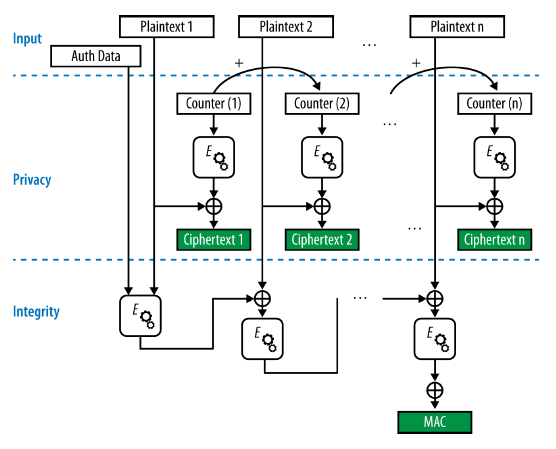
\includegraphics[width=0.6\textwidth]{CCMP.png}
    \end{figure}
    CCMP = CTR + CBC-MAC \\
    CTR (counter mode) - tryb szyfrowania \textbf{AES}, w którym wszystkie kroki można wykonywać równolegle
    CBC-MAC (Cipher Block Chaining Message Authentication Code) - technika konstruowania kodu uwierzytelniającego wiadomość (MAC). Wiadomość jest szyfrowana za pomocą algorytmu szyfru blokowego w trybie łączenia bloków szyfru (CBC) w celu utworzenia łańcucha bloków w taki sposób, że każdy blok zależy od prawidłowego zaszyfrowania poprzedniego bloku. Ta współzależność gwarantuje, że zmiana dowolnego bitu tekstu jawnego spowoduje zmianę końcowego zaszyfrowanego bloku w sposób, którego nie można przewidzieć bez znajomości klucza do szyfru blokowego
    \item WPA-PSK (Wi-Fi Protected Access Pre-Shared Key), 4-way handshake \\
    WPA to protokół zabezpieczeń sieci Wi-Fi z silnym algorytmem szyfrowania oraz uwierzytelnianiem użytkownika.
    WPA-PSK to wersja protokołu WPA ze współdzielonym kluczem. Wszystkie podłączone stacje wykorzystują jeden wspólny klucz do autoryzacji i szyfrowania transmisji.
    \begin{figure}[H]
        \centering
        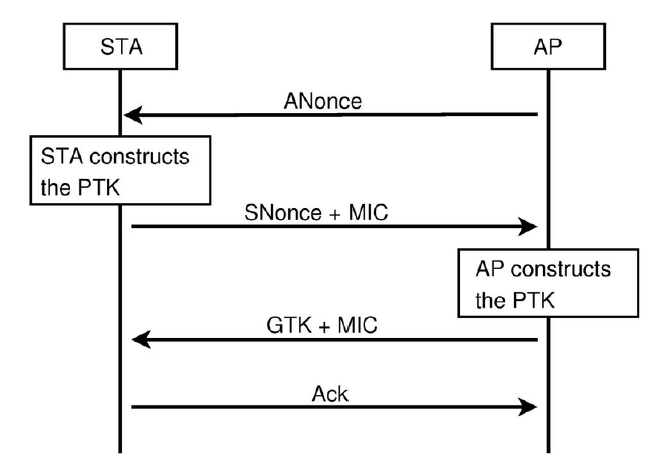
\includegraphics[width=0.6\textwidth]{WPASK.png}
    \end{figure}
    PTK = Hash(Key, ANonce, SNonce, APMAC, STAMAC)
    \item WPA-Enterprise \\
    system zabezpieczeń oparty na uwierzytelnianiu klucza za pomocą serwera RADIUS,
    co często wiąże się z koniecznością posiadania odpowiedniego certyfikatu. W przeciwieństwie do WPA-PSK każdy użytkownik dostaje oddzielny klucz.
    \item SAE (Diffie-Hellman) w WPA3 (Simultaneous Authentication of Equals) \\
    mechanizm równoczesnego uwierzytelniania równych stron, pozwalający zapobiegać ujawnieniu komunikacji klienta, kiedy hasło zostanie odgadnięte (np. brute forcem).
\end{itemize}
\subsection{Inne sieci bezprzewodowe}
\begin{itemize}
    \item LTE (Long Term Evolution) \\
    standard przesyłu danych w sieci 4g
    \item Ad-hoc \\
    struktura sieci bezprzewodowej bez centralnego punktu dostępu
    \item Sensor networks sieć czujników komunikujących się między sobą i / lub przesyłających dane do wspólnego punktu
    \item Bluetooth \\
    standard bezprzewodowej komunikacji krótkiego zasięgu
    \item Zigbee \\
    protokół transmisji danych w sieci bezprzewodowej (np. mesh, cluster tree). Podobny do Wi-Fi, ale zużywa mniej energii. Ma zasięg do 100 km.
\end{itemize}

\label{sec:warstwa-sieci}
\section{Warstwa sieci (warstwa internetu)}
\begin{itemize}
    \item Adresowanie \\
    obliczanie adresów \\
    MAC $\rightarrow$ druga warstwa OSI \\
    IP $\rightarrow$ trzecia warstwa OSI
    \item Trasowanie \\
    wyznaczanie trasy \\
    Jaki powinien być algorytm trasowania? \\
    Jakie cele optymalizować? \\
    Jak zainicjalizować algorytm? \\
    Czy i jak go dostosowywać do sytuacji?
    AS - \\
    IGP (Interior Gateway Protocol) \\
    - RIP (Routing Information Protocol) (Distance Vector) \\
    - OSPF (Open Shortest Path First) (Link State) \\
    EGP (Exterior Gateway Protocol) \\
    - BGP (Border Gateway Protocol)
    \item Połączenia \\
    Inicjalizacja trasy \\
    Adresowanie \\
    Stan trasy \\
    Alokacja przepustowości \\
    Transmisja pakietowa
    \item Łączenie różnych sieci \\
    Tłumaczenie adresów \\
    ARP (Address  Resolution Protocol) - wykorzystywany, kiedy znany jest adres IP adresata, a potrzebny adres MAC (np. W sieciach lokalnych). Nadawca broadcastuje IP adresata z zapytaniem, czyj jest ten adres, a adresat odsyła w odpowiedzi swój adres MAC (translacja). \\
    Tłumaczenie wiadomości
    \item Wielu adresatów \\
    unicast, czyli one-to-one (karty Ethernet) \\
    multicast, czyli one-to-many (jeden grupowy odbiorca - host group) \\
    broadcast, czyli one-to-all \\
    anycast, czyli one-to-nearest-one
    \item Panowanie nad buforami \\
    Nadawca i odbiorca mają bufory. Nadawca może opróżnić swój dopiero po otrzymaniu potwierdzenia odbioru. Przy każdym potwierdzeniu dostaje też informacje o rozmiarze okna odbiorcy. \\
    Router z nieograniczonym buforem $\implies$ nieograniczone opóźnienia (dlaczego?)\\
    Router z dużym buforem i mechanizm TTL $\implies$ zerowa przepustowość \\
    Mechanizm TTL - \\
    Kiedy bufor zbliża się do zapełnienia, lepiej sprawdza się usunięcie losowego bufora niż najstarszego. Wtedy bardziej narażony na straty jest ten, który wysyła najwięcej pakietów
    Prealokacja zasobów \\
    Współpraca z wyższymi warstwami \\
    ECN (Explicit Congestion Notification) informuje nadawcę o zatorze, żeby podjąć odpowiednie działania. Oznacza pakiety poprzez odwrócenia bitu nagłówków. Hipotetyczna sytuacja: \\
    $\rightarrow$ X wysyła kopertę do Z dwa domy od niego. \\
    $\rightarrow$ X przekazuje kopertę pośrednikowi Y. \\
    $\rightarrow$ Jeśli Y jest zatłoczony, to stawia krzyżyk w rogu koperty i przekazuje ją dalej. \\
    $\rightarrow$ Kiedy Z otrzymuje kopertę i odnotowuje krzyżyk, to wie, że u któregoś z pośredników jest tłoczno. \\
    $\rightarrow$ Z wysyła ACK do X, również oznaczając je krzyżykiem i w ten sposób X też wie o zatorze.
\end{itemize}

\noindent
\textbf{QoS (Quality of Service)} - charakterystyka usługi komunikacyjnej obejmująca następujące mechanizmy
kształtowanie i ograniczanie przepustowości:
\begin{itemize}
    \item Zapewnianie sprawiedliwego dostępu do zasobów
    \item Nadawanie odpowiednich priorytetów pakietom wędrującym przez sieć
    \item Zarządzanie opóźnieniami w przesyle danych
    \item Zarządzanie buforowaniem nadmiarowych pakietów (DRR, WFQ, WRR) \\
    DDR (Deficit Round Robin) - mechanizm zarządzania pamięcią \\
    WRR (Weighted Round Robin) - mechanizm zarządzania pakietami \\
    WFQ (Weighted Fair Queuing) - mechanizm zarządzania przepływami w oparciu o przpisane im wagi
    \item Określenie charakterystyki gubienia pakietów
    \item Unikanie przeciążeń (CAC, UPC) \\
    CAC - Connection Admission Control \\
    UPC - Usage Parameter Control \\
\end{itemize}
\textbf{RED (Random Early Detection)} - algorytm kolejkowania oraz unikania zakleszczeń. W tradycyjnym algorytmie router lub inne urządzenie sieciowe buforuje tyle pakietów, ile tylko może, a resztę po prostu odrzuca.

\subsection{Adresy IP}
0.0.0.0/8 Current network \\
127.0.0.0/8 Loopback \\
10.0.0.0/8 Private network \\
172.16.0.0/12 Private network \\
192.168.0.0/16 Private network \\
192.88.99.0/24 IPv6 to IPv4 relay \\
224.0.0.0/4 IP Multiticast \\
255.255.255.255 Broadcast \\

\noindent
Maska określa, które bity muszą się zgadzać. \\
Multicasty są realizowane poprzez zakładanie wirtualnego adresu IP dla całej grupy odbiorców. \\
Zasięg adresów zaczynających się od 10 jest ograniczony do sieci prywatnej. Dlatego można nadać taki sam numer wielu urządzeniom, jeśli tylko są w różnych sieciach prywatnych. \\
Adresy są globalnie zarządzane przez IANA. Organizacja sprzedaje paczki adresów organizacjom na dany region świata. \\

\noindent
\textbf{CIDR} - \\
\textbf{AS} - \\

\subsection{Protokoły towarzyszące IP}
\begin{itemize}
    \item ARP (Address Resolution Protocol) \\
    protokół do mapowania logicznych adresów warstwy sieciowej na fizyczne adresy warstwy łącza danych
    \item DHCP (Dynamic Host Configuration Protocol) \\
    protokół komunikacyjny umożliwiający hostom uzyskanie od serwera danych konfiguracyjnych, np. adresu IP hosta
    \item ICMP (Internet Control Message Protocol)
    protokół do diagnostyki sieci i trasowania. Kontroluję transmisje danych.
    \item IGMP (Internet Group Management Protocol) \\
    protokół do zarządzania grupami multicatowymi

\end{itemize}
\noindent
Gdzie to można zobaczyć? \\
\href{https://www.iana.org/numbers}{https://www.iana.org/numbers} \\
whois \\
\href{https://stat.ripe.net}{https://stat.ripe.net}

\section{TCP}
Połączeniowy, niezawodny, strumieniowy protokół do przesyłania sieciowego, operuje w warstwie transportowej OSI.
\subsection{Nagłówek}
\begin{figure}[H]
    \centering
    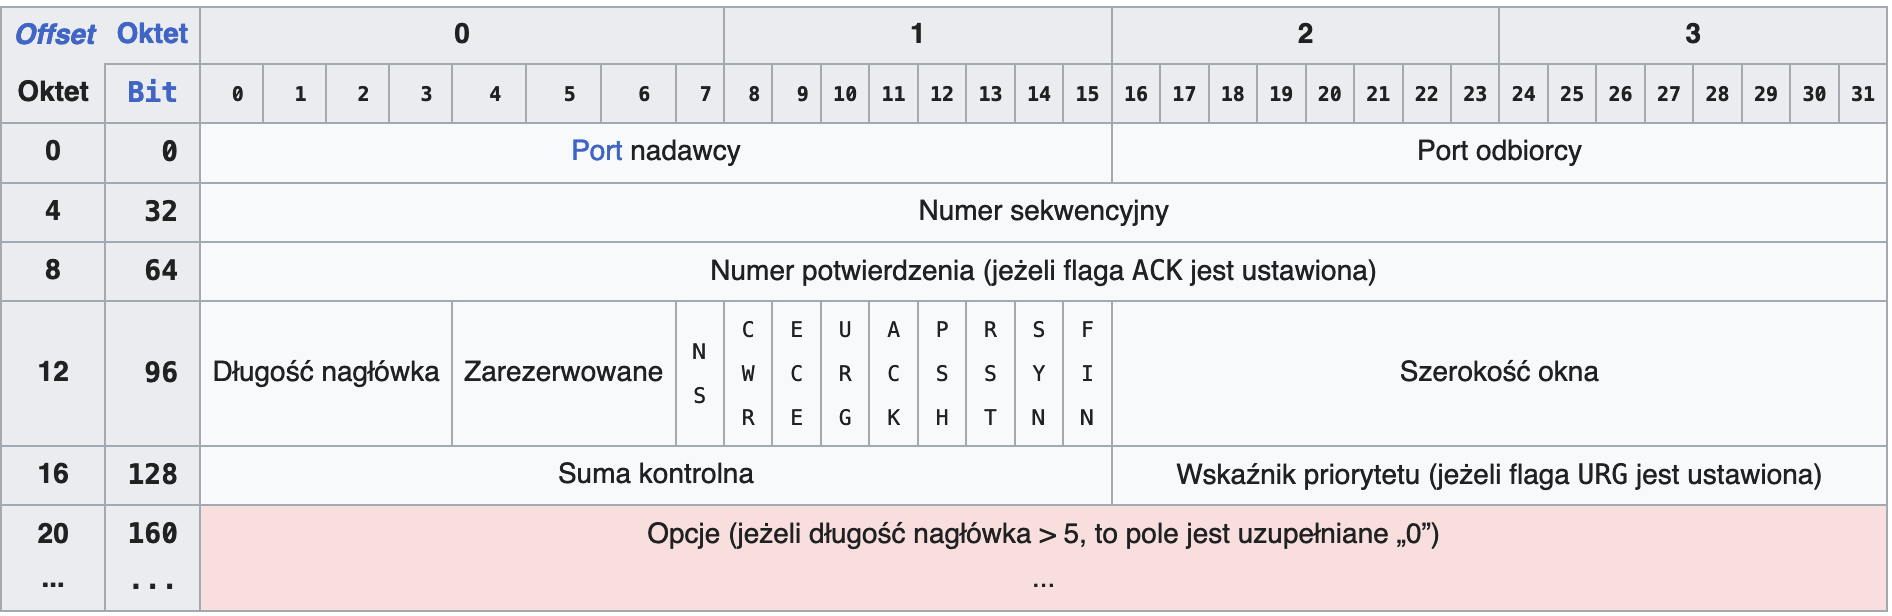
\includegraphics[width=0.8\textwidth]{tcp.png}
\end{figure}
\subsection{Sposoby na niezawodny transport}
\subsubsection{Niezawodne łączę}
\subsubsection{Łącze z błędami, ale bez traconych pakietów}
\begin{itemize}
    \item Potwierdzenia transmisji
    \item Retransmisje
    \item Błędy w potwierdzeniach
\end{itemize}
\subsubsection{Łącze z błędami i traconymi pakietami}
\subsection{Cechy TCP}
\begin{itemize}
    \item Podczas transmisji między hostami utrzymywane jest wirtualne trwałe połączenie
    \item Zapewnia niezawodny transfer danych, dzięki potwierdzaniu dostarczenia i retransmisji zgubionych pakietów
    \item Transmisja jest dwustronna (w jedną stronę dane, w drugą potwierdzenia)
    \item Radzi sobie z niepoprawną kolejnością
    \item Steruje przepływem, zapewniając, że nie przeciąży odbiorcy dzięki mechanizmowi \emph{sliding window}. TCP wysyła tylko tyle pakietów ile zmieści się w tym momencie w buforze użytkownika, kiedy wiadomość jest przetworzona to wysyłany jest ACK tej wiadomości wraz z aktualnym rozmiarem bufora.
    \item Ma uzgadnianie tożsamości poprzez handshake \ref{handshake}
    \item W celu weryfikacji wysyłki i poprawności datagramu używa sum kontrolnych
    \item Zakończenie połączenia może być zainicjowane przez dowolną stronę, wysyłany jest pakiet z flagą FIN. Operacja ta wymaga potwierdzenia pakietem z flagą FIN-ACK, w awaryjnych przypadkach można też zakończyć połączenie flagą RST (reset), co nie wymaga potwierdzenia.
\end{itemize}
\subsection{Stany połączenia}
Połączenie może znajdować się w jednym z 11 stanów. 
\begin{multicols}{2}
\begin{itemize}
    \item \textbf{LISTEN}
    \item \textbf{SYN-SENT}
    \item \textbf{SYN-RECEIVED}
    \item \textbf{ESTABLISHED}
    \item \textbf{FIN-WAIT-1}
    \item \textbf{FIN-WAIT-2}
    \item \textbf{CLOSE-WAIT}
    \item \textbf{CLOSING}
    \item \textbf{LAST-ACK}
    \item \textbf{TIME-WAIT}
    \item \textbf{CLOSED},
\end{itemize}
\end{multicols}
\subsection{Potrójny uścisk dłoni (three-way handshake)}
\label{handshake}
\begin{itemize}
    \item Pierwsze urządzenie wysyła drugiemu wiadomość SYN (synchronize), z własnym numerem $x$
    \item Drugie urządzenie odpowiada wiadomością SYN-ACK, z własnym numerem $y$ i potwierdzającym $x+1$
    \item Pierwsze urządzenie odpowiada wiadomością ACK, z numerem potwierdzającym $y+1$
    \item Drugie już nie odpowiada, synchronizacja zakończona
\end{itemize}
\begin{center}
    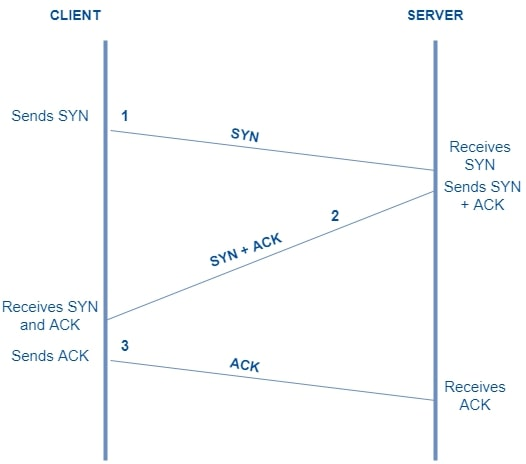
\includegraphics[width=0.5\textwidth]{handshake.jpg}
\end{center}
\subsection{Slow Start}
\begin{wrapfigure}{r}{0.4\textwidth}
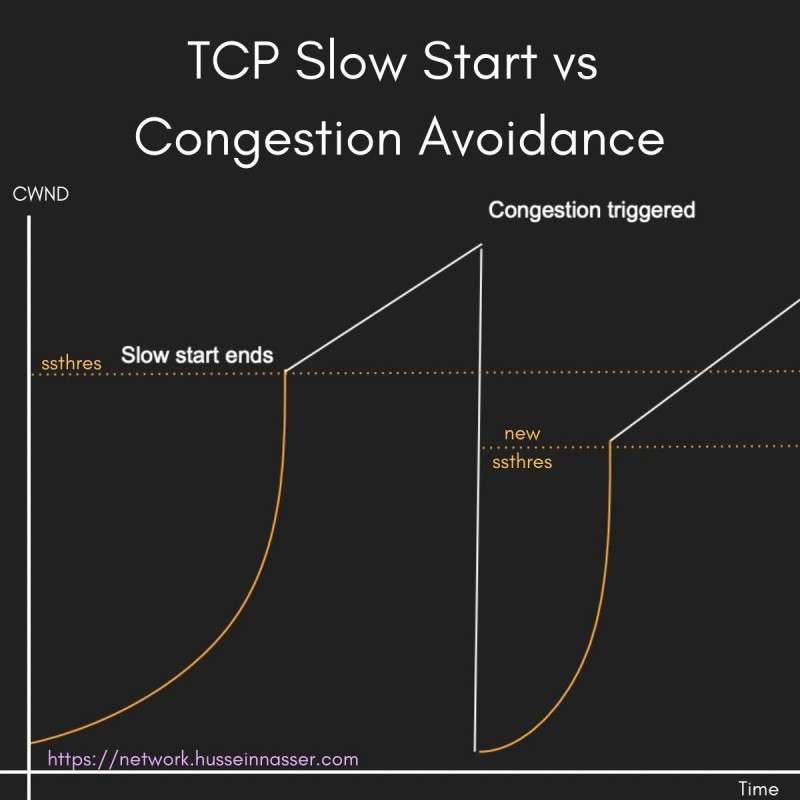
\includegraphics[width=\linewidth]{slow-start.jpg} 
\end{wrapfigure}
\textbf{Slow start} to algorytm na kontrole szybkości transmisji, gdy nie znamy prędkości łącza. Zaczynamy od bardzo powolnego przesyłu i zwiększamy jego prędkość, póki dostajemy poprawne potwierdzenie jej otrzymania. Kiedy jej nie dostaniemy to zmniejszamy prędkość. Najczęściej implementowane poprzez bin-search. Nie jest idealne, ale działa bardzo dobrze kiedy wszyscy użytkownicy sieci się do tego stosują, gdyż dzieli wtedy łącze po równo.\\
\subsection{Kontrola rozmiaru buforów}
\textbf{Warianty TCP:}
\begin{itemize}
    \item TCP Tahoe
    \item TCP Reno
    \item TCP Vegas
\end{itemize}
\subsection{Egzaminogenne ciekawostki}
\begin{itemize}
    \item Lepiej wysyłać duże segmenty. Nagle.
    \item Według standardu można wysyłać priorytetowe segmenty, jednak jest to archaizm, i większość implementacji nie traktuje ich inaczej.
\end{itemize}
\subsection{warianty}
\begin{itemize}
    \item \textbf{TCP Tahoe} = Slow Start + AIMD + Fast Retrasmit
\end{itemize}
\section{UDP}
Protokół stosowany w warstwie transportowej OSI, nie gwarantuje dostarczenia datagramu.
\subsection{Nagłówek}
Nagłówki są bardzo proste. Port nadawcy i suma kontrolna są opcjonalne, ale bez sumy kontrolnej nie możemy sprawdzić poprawności.
\begin{figure}[H]
    \centering
    \includegraphics[width=0.6\textwidth]{udp.png}
\end{figure}
\subsection{Zastosowania}
\begin{itemize}
    \item DHCP - Protokół umożliwiający hostom uzyskania od serwera danych konfiguracyjnych. Musi używać UDP bo w momencie gdy prosimy serwer o te dane nie mamy jeszcze nadanego adresu IP, a TCP wymaga posiadania stałego adresu IP.
    \item DNS - używa UDP po komunikacje są małe i muszą być wysłane jak najszybciej to możliwe
\end{itemize}
\section{Różnice między TCP a UDP}
Są używane w różnych scenariuszach, TCP znacznie popularniejszy
\begin{enumerate}
    \item \textbf{Prędkość} UDP znacznie szybszy od TCP.
    \item \textbf{Połączenie} 
    \begin{itemize}
        \item TCP jest zorientowany na połączenie, podczas wysyłania danych trwa ciągła komunikacja
        \item UDP wysyła wszystko jak leci, bez zastanowienia
    \end{itemize}
    \item \textbf{Gwarancje i kolejność pakietów}
        \begin{itemize}
        \item TCP gwarantuje pełność i odpowiednią kolejność pakietów
        \item W UDP dane mogą przyjść w złej kolejności, albo nawet wcale
    \end{itemize}
    \item \textbf{Zastosowania}
        \begin{itemize}
        \item TCP używane wszędzie, gdzie potrzebne jest niezawodne połączenie i gwarancja poprawności danych
        \item UDP jest używane, gdy zależy nam na przesyle o jak najmniejszym opóźnieniu, używany przede wszystkim w streamingu wideo i grach online, dla których utrata pojedynczego pakietu nie jest istotna
    \end{itemize}
    \item Większość implementacji faworyzuje transfer TCP nad UDP
\end{enumerate}
\section{HTTP}
HTTP - (z ang. Hypertext Transfer Protocol) - protokół do komunikacji w sieci WWW, służy do komukacji między użytkownikiem a serwerem, oparty na TCP. Domyślnie działa na porcie 80 (HTTPS na 443).
\subsection{Metody HTTP}
\begin{multicols}{2}
\begin{itemize}
    \item \textbf{GET}
    \item \textbf{HEAD}
    \item \textbf{PUT}
    \item \textbf{POST}
    \item \textbf{DELETE}
    \item \textbf{OPTIONS}
    \item \textbf{TRACE}
    \item \textbf{PATCH}
\end{itemize}
\end{multicols}

\subsection{Nagłówki}
W nagłówkach zawieramy dodatkowe informacje, takie jak data, język, typ danych czy informacje o hoście, aktualnie typów nagłówków jest bardzo dużo, w HTTP/1.0 tylko 14.\\
\textbf{Nagłówki w HTTP/1.0}
\begin{multicols}{2}
\begin{itemize}
    \item \textbf{Date}
    \item \textbf{Pragma} - zależne od implementacji
    \item \textbf{Authorization} - hasło uwierzytelniające
    \item \textbf{From} - adres email proszącego o dane (archaizm)
    \item \textbf{If-Modified-Since} - prosi o przesłanie dokumenty tylko jeśli był zmodyfikowany od podanej daty, używany do cache'owania
    \item \textbf{Referer} - adres strony, z której było przekierowanie
    \item \textbf{Server} - identyfikuje serwer i użyte w nim oprogramowanie
    \item \textbf{WWW-Authenticate} - określa sposób w jaki ma zostać przeprowadzone uwierzytelnienie użytkownika
    \item \textbf{Allow} - określa metody http obsługiwane przez serwer
    \item \textbf{Content-Encoding} - podaje format kompresji treści
    \item \textbf{Content-Length} - długość w bajtach przesyłanej wiadomości, dla danych przesyłanych z serwera obowiązkowy
    \item \textbf{Content-Type} - w jakim formacie jest dokument (html, pdf i.t.d.)
    \item \textbf{Expires} - data, po której dokument jest nieaktualny, używany do cache'owania
    \item \textbf{Last-Modified} - data ostatniej modyfikacji, używany do cache'owania
\end{itemize}
\end{multicols}
\subsection{Statusy}
Na zapytanie dostajemy od serwera odpowiedź z kodem statusu i opcjonalnie z jakimś plikiem (jeśli się wszystko powiodło)\\
\textbf{1xx} oznaczają, że serwer otrzymał poprawny request, i jeszcze go nie prze-procesował\\
\textbf{2xx} Sukces, robię to co mi kazano\\
\textbf{3xx} Przekierowania\\
\textbf{4xx} Błąd po stronie klienta\\
\textbf{5xx} Błąd po stronie serwera\\
\textbf{Przykładowe, i najczęściej używane statusy}\\\\
\begin{multicols}{2}
\begin{itemize}
    \item 200 OK
    \item 201 Created
    \item 202 Accepted
    \item 204 No Content
    \item 301 Moved Permanently
    \item 302 Moved Temporarily
    \item 304 Not Modified
    \item 400 Bad Request
    \item 401 Unauthorized
    \item 403 Forbidden
    \item 404 Not Found
    \item 418 I am a teapot
    \item 500 Internal Server Error
    \item 501 Not implemented
    \item 502 Bad Gateway
    \item 503 Service Unavailable
\end{itemize}
\end{multicols}

\subsection{Porównanie protokołów}
UDP jest szybszy niż TCP \\
TFTP(UDP) i HTTP(TCP) - różnie bywa, ponieważ TFTP zyskuje na tym, że UDP jest szybszy, ale same TFTP i HTTP są protokołami wyższej warstwy i zależą od warunków w sieci (przeciążenia, ilość danych do przesłania, itp.) \\
Potencjalne czynniki spowalniające
\begin{itemize}
    \item UDP  \\
    Pakiety mogą się gubić.
    \item TCP \\
    Wykorzystuje mechanizm sliding widow, co może ograniczać maksymalny rozmiar przesyłanych na raz danych. \\
    Wymaga mechanizmu potrójnego uścisku dłoni do nawiązania połączenia. \\
    \item HTTP \\
    Nagłówki do przesyłanych danych mogą być całkiem spore (informacje o cookies, itp.). \\
    Wymaga dodatkowego nakładu czasu (pewnie niewielkiego) przy nawiązywaniu połączenia związanego z wymogami protokołu TCP.
    \item TFTP \\
    Maksymalny rozmiar pakietu do wysłania na raz to 512B. \\
    Po każdym pakiecie trzeba poczekać na ACK, zanim zostanie wysłany kolejny.
\end{itemize}

\subsection{Serwery wirtualne}
Można hostować więcej niż jedną domenę na jednym serwerze. Trzeba wtedy dla każdej wiadomości przychodzącej/wychodzącej z serwera ustawić stosowny nagłówek \textbf{HOST}, jest on tak czy siak wymagany od HTTP/1.1.
\subsection{Ciasteczka (cookies)}
Pliki cookie są zapisywane na maszynie klienta i przy niektórych requestach wysyłane z powrotem do hosta aby dostać jakieś spersonalizowane dane. Używane często do implementacji systemu logowania i utrzymywania sesji. Żeby je zapisać, serwer wysyła request z nagłówkiem \textbf{Set-Cookie}, a żeby je wysłać z powrotem, do requesta dołączamy odpowiedni nagłówek \textbf{Cookie}
\subsection{Utrzymywanie połączenia}
W wersjach HTTP/1.1 i nowszych może być utrzymywane stałe połączenie TCP, które zamykane jest kiedy, któraś ze stron wyśle request z nagłówkiem 'Connection: close', włączamy tą opcję dodając do wiadomości nagłówek 'Connection: keep-alive', przydatne jeśli planujemy robić dużo requestów w krótkim czasie.
\subsection{Wysyłanie tylko części pliku}
\subsubsection{range}
Przy pomocy nagłówka \textbf{range} możemy poprosić serwer o dosłanie tylko części pliku, przydatne kiedy plik jest duży i chcemy usprawnić ładowanie, można poprosić o wiele części na raz. Serwer odsyła nam częściowy plik wraz ze statusem 206 - Partial Content, jeśli wyszliśmy poza zakres dostaniemy status 416 - Range not satisfiable.
\subsubsection{chunk}
Możemy także przy pomocy nagłówka \textbf{Transfer-Encoding: chunked} wysłać plik w chunkach, przydatne jeśli plik jest generowany dynamicznie. Pomijamy wtedy nagłówek 'Content-Length'
\subsection{Negocjacja zawartości}
\subsection{Trzeba trzymać standardy}
Metoda \textbf{options} to prośba o przesłanie informacji na temat dostępnych metod komunikacji.
\section{Bezpieczeństwo i poufność}
\subsection{Rodzaje zagrożeń}
\begin{itemize}
    \item Podglądanie
    \item Modyfikacja, usuwanie komunikatów
    \item Blokowanie komunikacji
\end{itemize}
\subsection{Hasze kryptograficzne}
\begin{itemize}
    \item \textbf{MD4} - została złamana i można wygenerować kolizję w czasie rzędu sekund, przez to wyparta przez MD5, która jest jej następnikiem.
    \item \textbf{MD5} - z ciągu danych o dowolnej długości generuje 128 bitowy hasz, znaleziono sposób na generowanie kolizji, jednak i tak jest użyteczna w niektórych zastosowaniach. 
    \item \textbf{SHA1} tworzy 160 bitowy hasz z wiadomości o rozmiarze maksymalnym $2^64$ bitów, ciężki do złamani, jednak powoli się nad tym pracuje więc w nowych aplikacjach lepiej używać SHA2.
    \item \textbf{SHA2} - Następnik SHA1 składa się z zestawu czterech funkcji generujących odpowiednio 224, 256, 384 lub nawet 512 bitowe hasze, ma podobną implementacje co SHA1.
    \item \textbf{SHA3} - wyłoniony w 2012 w konkursie następnik SHA2, działa na bazie algorytmu Keccak. Ma zupełnie inną budowę niż SHA2 dzięki czemu jest znacznie wydajnieszy zachowując zbliżone parametry bezpieczeństwa.
\end{itemize}
\subsection{Szyfrowanie symetryczne}
Algorytmy symetryczne do szyfrowania i deszyfrowania informacji używają tego samego klucza, lub takich dwu kluczy, z których mając jeden można jednoznacznie wyznaczyć drugi. Szyfrując wiadomość wynikowy szyfr jest równy na długość wiadomości. Dzielą się na \textbf{szyfry strumieniowe}, gdzie przetwarzamy informacje bit po bicie i \textbf{blokowe} gdzie szyfrujemy naraz bloki danych i potem je sklejamy.
\
\begin{itemize}
    \item \textbf{XOR} - xorujemy z kluczem. Często używany w połączeniu z innych szyfrem. Jest ekstra bo jest idealnie zbalansowany, każdy bit ma statystycznie równe szanse stać się 0 jak i 1. 
    \item \textbf{AES} - Szyfr blokowy, o rozmiarze bloku 128 bitów, bardzo bezpieczny, zoptymalizowany pod szybkość działania i niskie zużycie pamięci, standard do szyfrowania tajnych informacji przez agencje wywiadowcze.
    \item \textbf{CBC} - (z ang. Cipher Block Chaining) tryb pracy szyfrów blokowych, gdzie każdy blok jest przez zaszyfrowaniem jest xorwany z szyfrem poprzedniego bloku.
    \item \textbf{CTR}
    \item \textbf{Diffie-Hellman}
    \item \textbf{Needham-Schroeder}
    \item \textbf{Needham-Schroeder (Kerberos style)}
\end{itemize}
\subsection{Szyfrowanie kluczem publicznym - RSA}
    RSA to najpopularniejszy asymetryczny algorytm kryptograficzny. Może być stosowany zarówno do szyfrowania jak i do podpisów cyfrowych. Jego bezpieczeństwo opiera się na trudności faktoryzacji dużych liczb. Na terenie USA opatentowany więc można go tam używać tylko do celów niekomercyjnych \textit{(america at its finest xdd)}\\
    \subsubsection{Generowanie kluczy}
    \begin{enumerate}
        \item Wybieramy losowo dwie duże liczby $p$ i $q$
        \item obliczamy $n=p*q$
        \item obliczamy $\lambda = NWW(p-1, q-1)$
        \item wybieramy liczbę $e$ względnie pierwszą z $\lambda$, z przedziału $(1,\lambda)$
        \item znajdujemy liczbę $d$, dla której $d*e \equiv 1 (mod \lambda)$
    \end{enumerate}
    \textbf{Szyfrowanie i deszyfrowanie}
    Dzielimy wiadomość na bloki a następnie szyfrujemy i deszyfrujemy każdy blok używając wzorów.
    \begin{multicols}{2}
        \begin{center}
            $c &\equiv m^e \pmod{n}$\\
            (szyfrowanie)
        \end{center}
        \begin{center}
            $m &\equiv c^d \pmod{n}$\\
            (deszyfrowanie)
        \end{center}
    \end{multicols}
    \subsubsection{Bezpieczeństwo}
    Im większe liczby wybierzemy tym trudniejszy jest do złamania. W 2020r. największy złamany klucz miał 829 bitów. Potencjalnym zagrożeniem dla RSA jest skonstruowanie stabilnego komputera kwantowego, gdyż w teorii mogą one z łatwością poradzić sobie z problemem faktoryzacji, jednak na razie ze względu na niestabilność największa zfaktoryzowana przez nie liczba ma zaledwie 72 bity.
\subsection{Autoryzacja}
\begin{itemize}
    \item \textbf{hasłem}
    \item \textbf{kluczem}
    \item \textbf{podpisanym kluczem}
\end{itemize}
\subsection{Podpis cyfrowy}
Cyfrowy podpis służy do stwierdzenia czy wiadomość pochodzi od właściwego nadawcy i nie została zmieniona podczas transmisji. Sprawdzamy czy szyfr wiadomości jest równy oczekiwanemu.
\subsubsection{PGP}
PGP (z ang. Preety Good Privacy) \sout{ma najlepszy skrót} jest jednym z najczęściej używanych programów do elektronicznego podpisywania, i szyfrowania plików. Używa RSA oraz DSA.
\subsection{SSL}
Protokół, który umożliwia bezpieczną komunikację w Internecie w ramach HTTPS, chroni dane w warstwie transportowej poprzez ich zaszyfrowanie, pozwala na weryfikacje tożsamości i zapewnia integralność danych. zapobiega atakom man in the middle. Używa do tego podpisów cyfrowych i haszowania za pomocą SHA2.
\subsubsection{Wystawianie certyfikatów}
Certyfikaty SSL strony uzyskują od urzędów certyfikacji na pewien okres czasu, po tym jak sprawdzą one w jakiś sposób (np. przez to, że uruchomimy jakiś skrypt je pingujący z serwera, do którego jest podpięta domena), naszą tożsamość. Wystawiają także specjalne certyfikaty prywatnym instytucją, które umożliwiają im podpisywanie kolejnych domen, tworzy się w ten sposób łańcuch certyfikatów, gdyż każdy certyfikat, aby móc potwierdzić jego autentyczność musi także podać certyfikat wystawiającego.
\subsubsection{Inicjacja połączenia}
\begin{enumerate}
    \item W trakcie handshake'u, serwer wysyła swój certyfikat SSL, albo ich łańcuch i użytkownik decyduje czy im ufać czy nie. Wysyła także informacje o metodzie szyfrowania, czasem też prosi klienta o jego certyfikat.
    \item Klien generuje klucz sesji, wysyła go serwerowi szyfrując go kluczem publicznym serwera, dzięki temu tylko serwer z jego unikalnym kluczem prywatnym może odszyfrować klucz sesji.
    \item Wysyłane są komunikaty potwierdzające pomyślne wymianę kluczami od teraz całość interakcji jest szyfrowana tajnym kluczem sesji.
\end{enumerate}
\section{Bezpieczne Sieci}
\textbf{\emph{Uwaga!!! Niedokończona sekcja, bo autor uznał, że musi się wyspać, tego i tak raczej nie będzie na egzaminie}}\\
\subsection{IPsec}
Zbiór protokołów służących do implementacji bezpiecznych połączeń obrazy wymiany kluczy szyfrowania. Polega na szyfrowaniu całego ruchu IP. Może być wykorzystany do tworzenia VPNów. 
\susubsection{IKE}
\textbf{IKE} (z ang. Internet Key exchange) polega na:
\begin{itemize}
    \item Uwierzytelnieniu obu stron, przez hasło, RSA, lub certyfikaty
    \item nawiązaniu bezpiecznego kanału IKE
    \item uzgodnienie bezpiecznych kluczy kryptograficznych oraz kanału do komunikacji.
\end{itemize}
Główną zaletą jest fakt, że nie trzeba ręcznie ustawia kluczy tylko ustalić wspólne hasło i samo się zrobi
\subsection{VPN}
\subsubsection{OpenVPN}
\section{Sieci P2P} 
\textbf{\emph{Uwaga!!! Niedokończona sekcja, bo autor uznał, że musi się wyspać, tego i tak raczej nie będzie na egzaminie}}\\
\subsection{BitTorrent}
protokół wymiany i dystrybucji plików przez Internet, którego celem jest odciążenie łączy serwera udostępniającego pliki. Jego największą zaletą w porównaniu do protokołu HTTP jest podział pasma pomiędzy osoby, które w tym samym czasie pobierają dany plik. Oznacza to, że użytkownik w czasie pobierania wysyła fragmenty pliku innym użytkownikom.
\\\\
\subsection{Torrentowe Pojęcia}
\textbf{Peer} - użytkownik, który w danym momencie pobiera i udostępnia dany plik.
\\
\textbf{Seeder} - użytkownik, który posiada kompletny plik i udostępnia go innym osobom.
\\
\textbf{Tracker} - serwer przekazujący informacje (adresy IP) o innych użytkownikach pobierających dany plik.
\\
\textbf{Plik .torrent} - metaplik zawierający niezbędne informacje (między innymi zawartość archiwum i adres trackera, sumy kontrolne plików) do
rozpoczęcia pobierania pliku.
\\
\textbf{Magnet} - typ linku URI używany w torrentach, który prowadzi do jakiegoś pliku, plik jest identyfikowany poprzez jego hasz, a nie lokalizacje czy nazwę
\subsubsection{DHT}
\paragraph{Rozproszona tablica mieszająca} (z ang. distributed hash table) służą w sieciach P2P do odszukania komputerów, na których znajduje się plik. 
Działa jak zwykła hasz mapa, ale przestrzeń adresowa jest rozrzucona po różnych komputerach, dobrze zaimplementowana jest jednak odporna na awarie urządzeń składowych.
\paragraph{Chord} protokół do implementacji DHT w sieci P2P. Przypisujemy każdemu wierzchołkowi (urzadzeniu) zestaw kluczy, który ma zapamiętać. Robimy cykl haszy, do którego wpinają się komputery losując hasz i przechodzimy po nim. Pamiętamy jump-pointery do kolejnych potęg dwójki, żeby było szybciej. Oczywiście część miejsc w naszym kółku będzie niezapełniona przez żadne urządzenie. 
\subsection{TOR}
Tor to sieć, która dzięki P2P zapewnia użytkownikom prawie anonimowy dostęp do zasobów, który nie podlega analizie ruchu sieciowego. Wielowarstwowo szyfruje komunikaty (stąd ta cebula w logo). Bazuje na protokole SOCKS, który polega na wymianę pakietów przy pośrednictwie serwera proxy.  Użytkownik musi mieć uruchomiony program, który łączy się z serwerem pośredniczącym (węzłem). Zwykle komunikacja przechodzi przez wiele węzłów przez co trudne jest ustalenie jej trasy.
\section{Przydasie}
\textbf{\emph{To są ostatnie laby, które autor pominął bo uczył się na probabila}}\\
\subsection{Openvpn}
\noindent
Uruchamianie seerwera OpenVPN: \\
\texttt{sudo openvpn server.ovpn} \\
Uruchamianie klienta OpenVPN: \\
\texttt{sudo openvpn client.ovpn} \\
Sprawdzanie połączenia: \\
\texttt{ping <server\_ip>} \\
\texttt{ping <client\_ip>} \\
Sprawdzanie przypisanego numeru IP: \\
\texttt{route -n} \\
Tu można sprawdzić nazwy urządzeń i potem wywołać \\
\texttt{ip addr show name}
\subsection{DNS}
\noindent
Żeby sprawdzić adres IP domeny można wykorzystać jedno z poleceń: \\
\texttt{nslookup <domain\_name>} \\
\texttt{dig <domain\_name>} \\
\end{document}